\documentclass[14pt]{extarticle}
\usepackage{extsizes}
\usepackage{geometry}
\geometry{margin=0.5in}

%% for images
\usepackage{graphicx}
\graphicspath{ {images/} }

%% language support
\usepackage[T1,T2A]{fontenc}
\usepackage[utf8]{inputenc}
\usepackage[english,russian]{babel}

\usepackage{amsmath}
\usepackage{tikz}

%% hyperrefs
\usepackage{hyperref}
\hypersetup{
    colorlinks,
    citecolor=black,
    filecolor=black,
    linkcolor=black,
    urlcolor=black
}

\title{2024}
\author{Death Sentence, 4th Term}
\begin{document}
\maketitle
\tableofcontents

\section{Основы ускорения вычислений на CUDA на Питоне.}
СUDA - специальный фреймворк для ускорения вычислений посредством
параллелизации на Nvidia GPU. \\
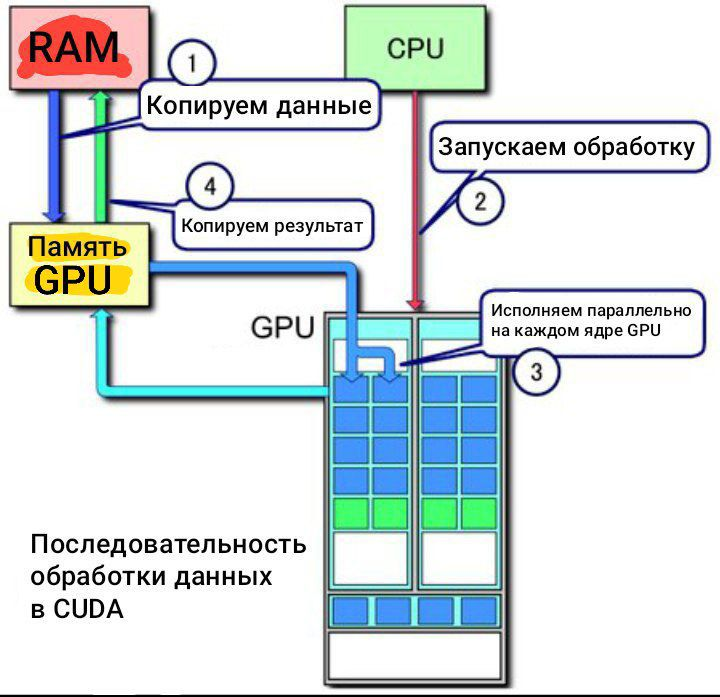
\includegraphics[scale=0.5]{CUDA_processing_flow.png}
\newpage
\subsection{Введение в CUDA питон с Numba}
Numba - JIT компилятор, преобразующий функции в более быстрые 
их варианты. Работает в основном с числовыми типами - int, float,
complex. Может использовать как CPU, так и GPU.
CPU-ускорение создаётся через декоратор @jit, который 
подключается как \begin{verbatim} from numba import jit \end{verbatim} 
Общая схема работы Numba такая:\\
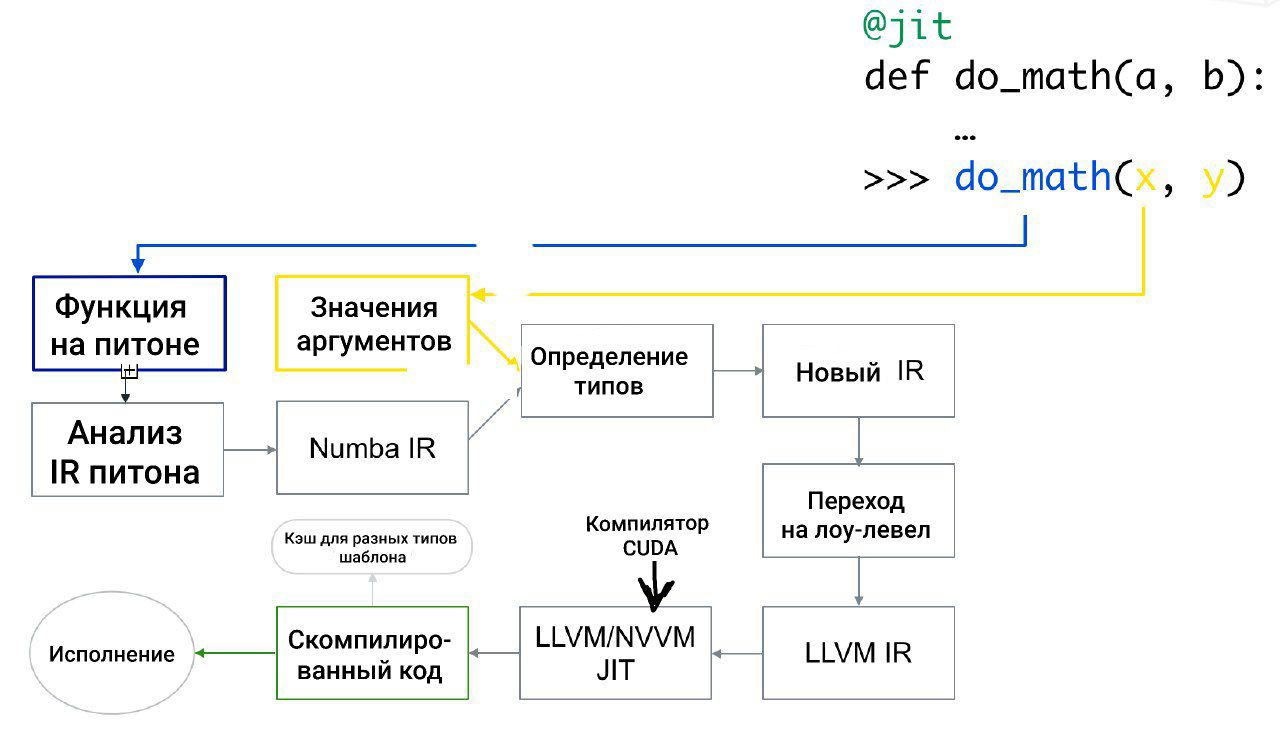
\includegraphics[scale=0.4]{numba.jpeg}
Здесь самое важное, что Numba может оптимизировать
далеко не все типы, как уже было сказано. Для выброса 
исключения о том, что тип не поддерживается, есть 
опция декоратора \begin{verbatim}nopython=True\end{verbatim},
она же по дефолту стоит в декораторе @njit. Если же
компилировать без неё, то Numba ничо не соптимизирует 
и это будет обычный питоновский код. Этот режим 
называется object mode, в отличие от nopython mode.
\newpage
Ура, GPU. Для CPU есть библиотека NumPy, 
предоставляющая интерфейс универсальных функций (ufunc), 
которые исполняют своё тело над каждым индексом в 
поданной на вход совокупности массивов. Естественно,
предполагается, что диапазон для 
итерирования для всех массивов совпадает.\\\\
Ufunc есть и в Numba, там они реализуются с помощью 
декоратора @vectorize, который исполняет
скомпилированные функции. Для GPU нужно указать в его 
аргументах желаемые сигнатуры функции и 
назначение (например, cuda). 
Нам интересна CUDA, и вот
что умеет делать Numba:\\
\begin{enumerate}
    \item Компилит так называемый CUDA kernel - 
    функция для GPU, которая будет параллелиться
    \item Выделяет память под входные и выходные данные
    \item Копирует входные данные в GPU
    \item Исполняет CUDA kernel 
    с заданной конфигурацией ядра GPU, основанной
    на размерах типов 
    \item Копирует данные назад на CPU 
    \item Возвращает результат типа NumPy array 
\end{enumerate}
Выглядит это всё довольно плохо и на малых данных 
влечёт за собой кучу оверхедов - вы видите, 
сколько тут лишних шагов. Оказывается, 
Big Data не так уж и бесполезны, да? GPU нужны
большие объёмы данных для организации работы
на своих сотнях и тысячах ядер. А ещё надо по 
возможности использовать 32-битные типы вместо 64,
потому что GPU чувствителен к вещам такого рода.\\
А ещё на GPU не работает половина NumPy, так что
нужно использовать math.\\\\
В лабе посмотрите, что для поэлементных функций это
в принципе нормально работает. Там как раз будет 
упражнение на это. Ещё раз, видим ПОЭЛЕМЕНТНО - 
используем vectorize. Поэлементно - значит, как минимум должен 
быть массив как аргумент.
\\\\
Но не все функции
в мире поэлементные, а оптимизировать надо всё. Для остальных 
функций есть @cuda.jit - ещё один декоратор, который имеет 
опцию device - она позволяет запретить исполнять 
функцию вне GPU. Ну и да, он компилит функции, 
тем самым ускоряя их работу. 
\\\\Кстати на GPU и 
питона то толком нет, поэтому код писать мы будем 
тупой.\\\\
Если бы мы были нормальными людьми, мы бы 
писали медленный, но простой код. Но нам придётся 
писать быстрый, а для этого кучу всего надо подкрутить
вручную.\\
Можно было заметить, что мы нигде явно не прописывали,
когда и как мы передаём данные между CPU и GPU. \\\\
Для того чтобы 
данные передавались только явно, 
мы используем специальный тип данных - device array. То, что в 
нём лежит, всегда находится на GPU. Инициализируется он функцией 
cuda.to\_device из CPU-шного массива либо создаётся пустым 
с помощью cuda.device\_array(shape, dtype). В CPU он передается 
по требованию с помощью copy\_to\_host.\\
Оптимизированная передача данных это круто, но вообще было бы неплохо
ещё и модифицировать данные внутри GPU, да? Для этого мы добавляем
в наши ufunc при вызове параметр out - device array, 
в который она положит свой результат -
используем её как процедуру. Также, ufunc неявно принимают
device array на вход вместо обычных массивов - исполняясь
на GPU, таким образом они работают уже с тем, что там лежит,
исключая лишнее копирование в GPU.\\
\\
Примечания для упражнений:\\
- Следите за типами!\\
- Проверяйте синтаксис\\
- По дефолту функции исполняются на CPU, если они не 
@vectorize и не @cuda.jit, поэтому стоит делать внутри 
функций всё через device array (который, кстати, можно 
переиспользовать)

\end{document}
